\documentclass{beamer} %
\usetheme{CambridgeUS}
\usepackage[latin1]{inputenc}
\usefonttheme{professionalfonts}
\usepackage{times}
\usepackage{tikz}
\usepackage{amsmath}
\usepackage{verbatim}
\usepackage{epstopdf}
\usetikzlibrary{arrows,shapes}
\usepackage[pscoord]{eso-pic}% The zero point of the coordinate systemis the lower left corner of the page (the default).

\newcommand{\placetextbox}[3]{% \placetextbox{<horizontal pos>}{<vertical pos>}{<stuff>}
  \setbox0=\hbox{#3}% Put <stuff> in a box
  \AddToShipoutPictureFG*{% Add <stuff> to current page foreground
    \put(\LenToUnit{#1\paperwidth},\LenToUnit{#2\paperheight}){\vtop{{\null}\makebox[0pt][c]{#3}}}%
  }%
}%

\author{M. Sakai}
\title{High Energy Imaging}
\date{March 19, 2013}

\begin{document}
\frame{\titlepage}
% For every picture that defines or uses external nodes, you'll have to
% apply the 'remember picture' style. To avoid some typing, we'll apply
% the style to all pictures.
\tikzstyle{every picture}+=[remember picture]

% By default all math in TikZ nodes are set in inline mode. Change this to
% displaystyle so that we don't get small fractions.
\everymath{\displaystyle}

\begin{frame}
\frametitle{Motivation}
	\begin{itemize}
		\item Utilize many photons at high energies to reconstruct event track shape.
		\item Reconstructing lepton direction gives handle on neutrino direction.
		\item lepton track shape gives handle on neutrino flavor.
		\item Use Fully contained events.
	\end{itemize}
\end{frame}

\begin{frame}{Where are They?}
	\begin{figure}
		\includegraphics[width=\textwidth,height=0.7\textheight,keepaspectratio]
			{material/high_energy_event_candidates_sanshiro.png}
		\caption{
			High ID PMT charge. Low OD hits.
		}
	\end{figure}
	%\placetextbox{.5}{.9}{\Huge\texttt{Sanshiro}}
\end{frame}

\begin{frame}{Diagram of Fermat Surface}
	\begin{figure}
		\includegraphics[width=\textwidth,height=0.7\textheight,keepaspectratio]
			{material/fermat_surface_diagram.png}
	\end{figure}
\end{frame}

\begin{frame}{Algorithm}
	\begin{itemize}
		\item Start with an initial guess of track direction.
		\item Center of $\frac{1}{time}$ to fit initial guess of beginning of track.
		\item Center of $\sqrt{charge}$ to fit initial guess of middle of track.
		\item Start with simple isotropic point source of light to test guess.
	\end{itemize}
\end{frame}

\begin{frame}{Algorithm}
	\begin{figure}
		\includegraphics[width=\textwidth,height=0.7\textheight,keepaspectratio]
			{material/center_of_one_over_time.png}
	\end{figure}
	\begin{itemize}
		\item Center of $\frac{1}{time}$ to fit initial guess of beginning of track.
		\item Center of $\frac{1}{time} = \frac{\frac{1}{t_1}x_1 +
			\frac{1}{t_2}x_2}{\frac{1}{t_1} + \frac{1}{t_2}} = \frac{1}{2}x_1$
			gives correct vertex.
	\end{itemize}
\end{frame}

\begin{frame}{Algorithm}
	\begin{figure}
		\includegraphics[width=\textwidth,height=0.7\textheight,keepaspectratio]
			{material/center_of_sqrt_of_charge.png}
	\end{figure}
	\begin{itemize}
		\item Center of $\sqrt{charge}$ to fit initial guess of middle of track.
		\item Center of $\sqrt{charge} = \frac{\sqrt{q_1}x_1 +
			\sqrt{q_2}x_2}{\sqrt{q_1} + \sqrt{q_2}} = \frac{1}{2}x_1$
			gives correct vertex.
	\end{itemize}
\end{frame}

\begin{frame}{Algorithm}
	\begin{itemize}
		\item Original algorithm by work left by D. Hellgartner.
		\item For given point x in detector: $h(x,t) = \sum\limits_{\#PMT}
		\theta(q_i-q_{threshold})f(\Delta{t},t)$
		where $f(\Delta{t},t) = (\Delta{t} - t)exp(-\frac{(\Delta{t} -
					t)^2}{2\sigma^2})$, and $\Delta{t} = t_{hit} - t_{TOF}$
		\item Figure of Merit for Point x:
		$\int\limits_{-\infty}^{\infty}|h(x,t)|^2dt$
		\item Fit 3d regression line to resulting 4d FOM plot above some
		threshold.
	\end{itemize}
\end{frame}

\begin{frame}{Simulation Test}
	\begin{itemize}
		\item Reconstruction algorithm was tested using KLG4sim.
		\item Energy = 1GeV
		\item Lepton flavor = $e^+$ and $\mu^-$
		\item Events uniformly distributed inside outer buffer oil.
		\item Fully contained events (All ID PMTs hit and OD hit < 5)
	\end{itemize}
\end{frame}

\begin{frame}{1GeV $e^+$}
	\begin{figure}
		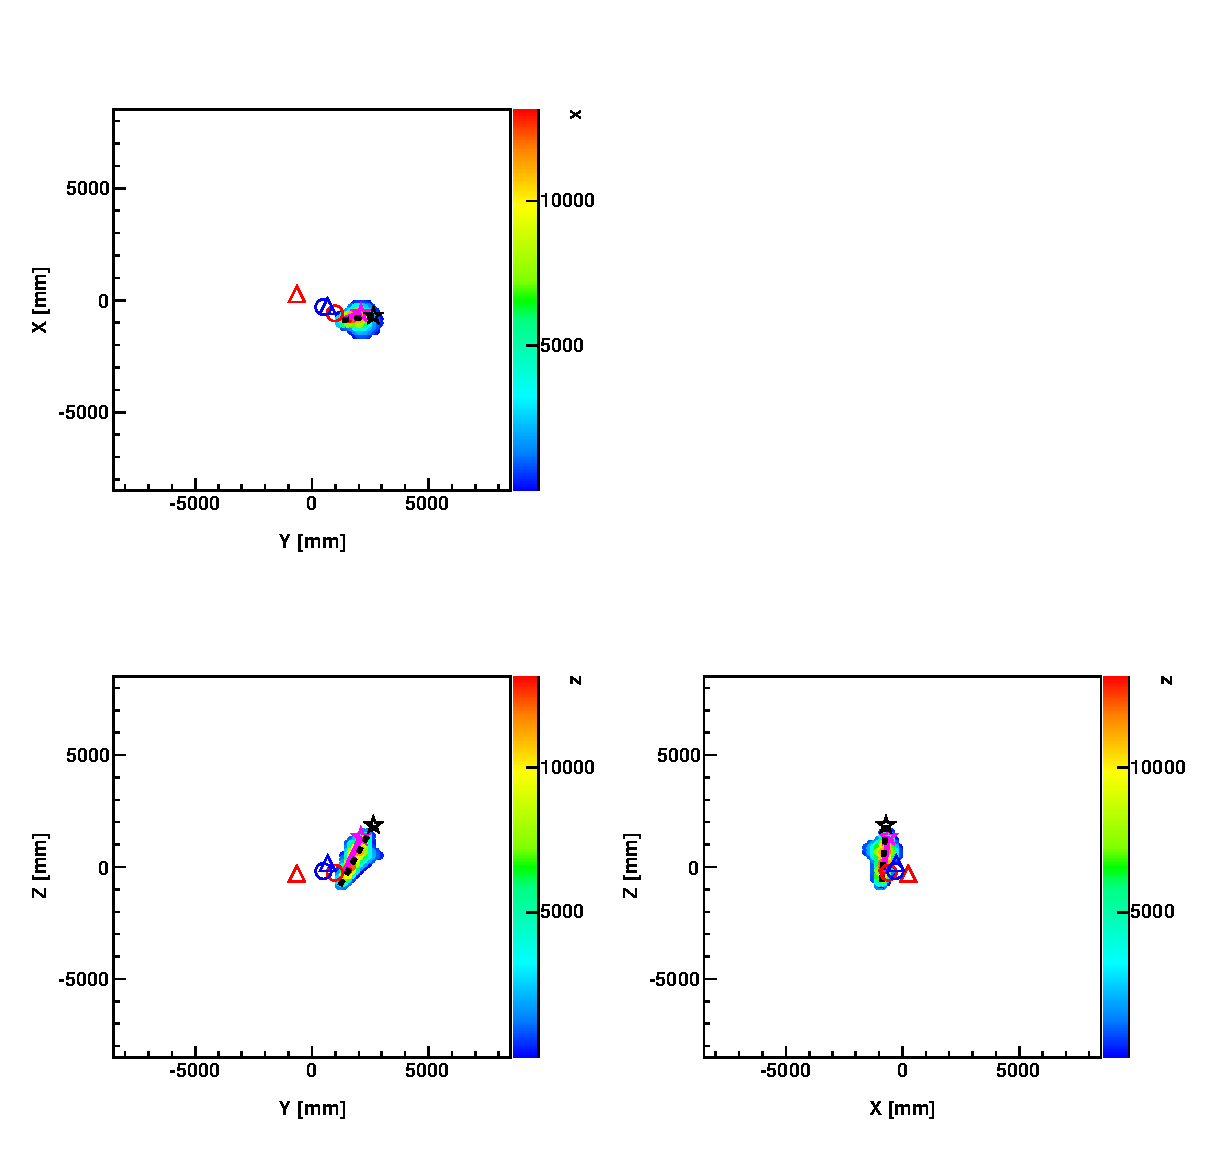
\includegraphics[width=\textwidth,height=0.9\textheight,keepaspectratio]
			{material/fom_map_e+_mtq_run0_evt472.pdf}
	\end{figure}
\end{frame}

\begin{frame}{1GeV $e^+$}
	\begin{figure}
		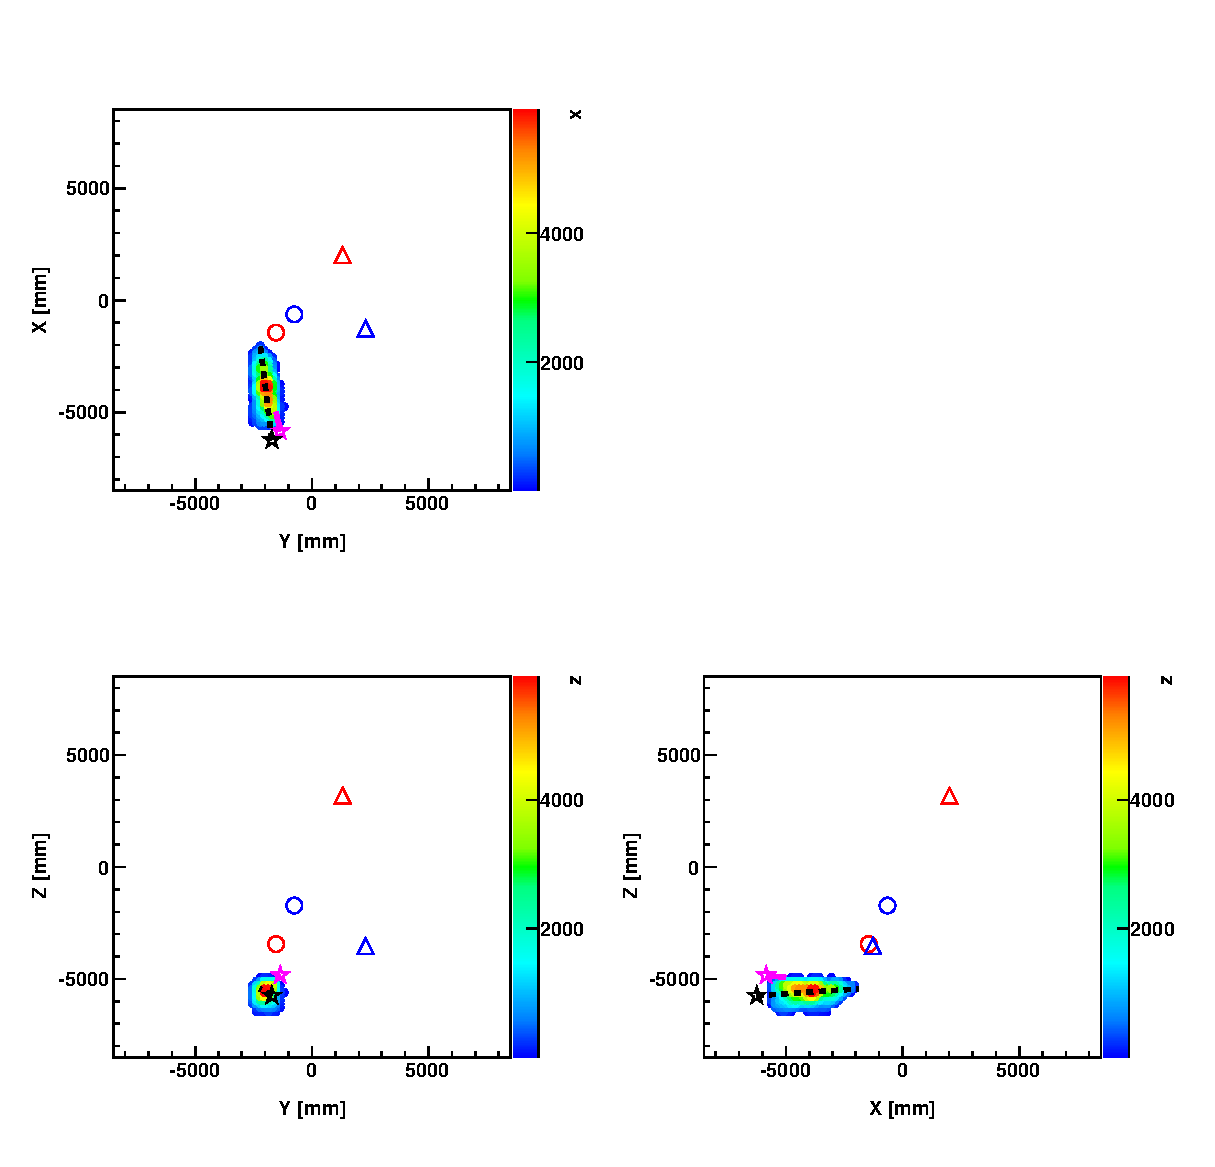
\includegraphics[width=\textwidth,height=0.9\textheight,keepaspectratio]
			{material/fom_map_e+_mtq_run0_evt566.pdf}
	\end{figure}
\end{frame}

\begin{frame}{Lepton Flavor Discrimination (No Cut)}
	\begin{figure}
		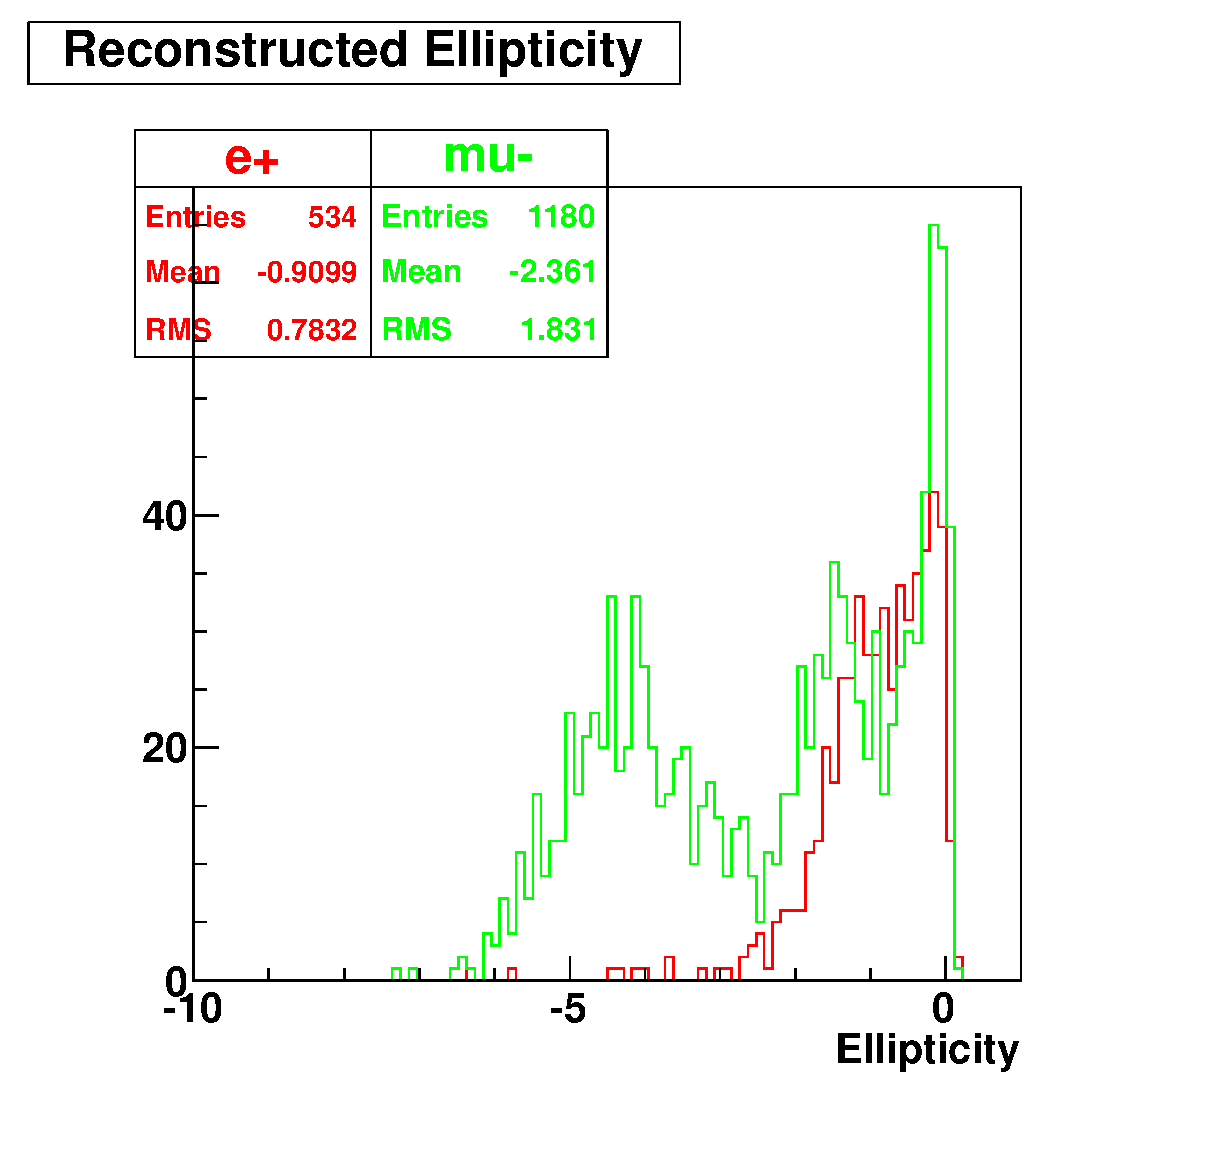
\includegraphics[width=\textwidth,height=0.9\textheight,keepaspectratio]
			{material/emu_mtq_recon_ellipticity-nocut.pdf}
	\end{figure}
\end{frame}

\begin{frame}{Lepton Flavor Discrimination (Track End 4m  Cut)}
	\begin{figure}
		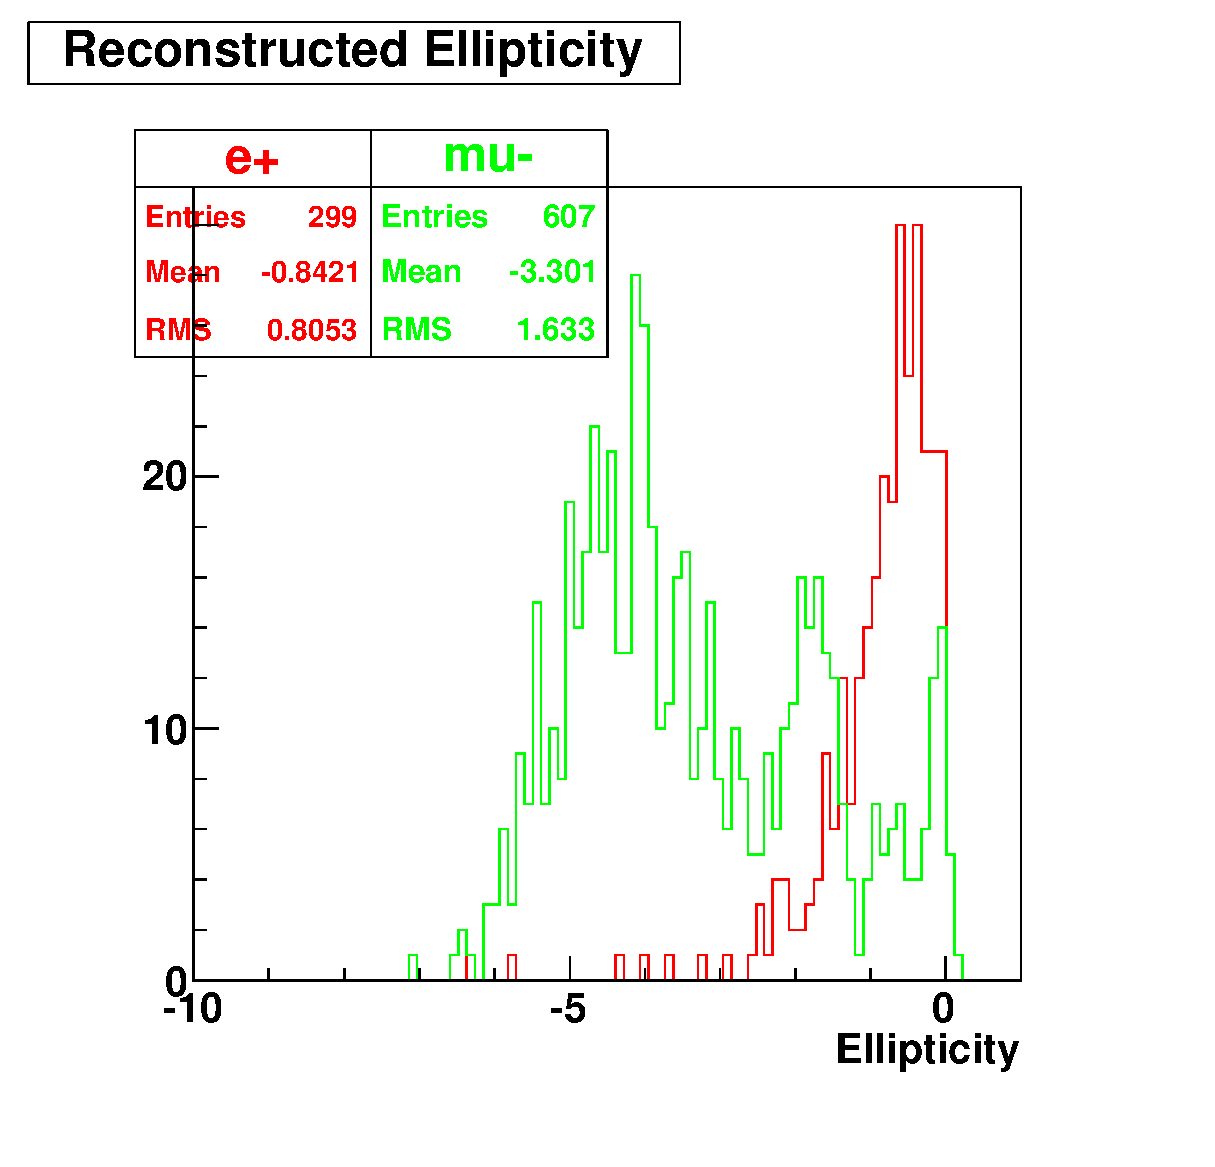
\includegraphics[width=\textwidth,height=0.9\textheight,keepaspectratio]
			{material/emu_mtq_recon_ellipticity-4Mcut.pdf}
	\end{figure}
\end{frame}

\begin{frame}{Lepton Flavor Discrimination (Track End 3m  Cut)}
	\begin{figure}
		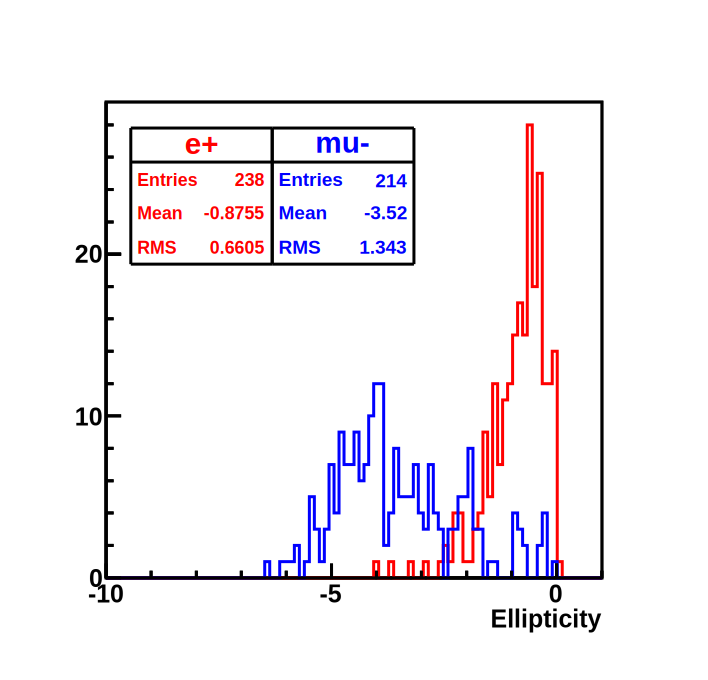
\includegraphics[width=\textwidth,height=0.9\textheight,keepaspectratio]
			{material/emu_mtq_recon_ellipticity-3Mcut.pdf}
	\end{figure}
\end{frame}

\begin{frame}{Reconstructed Angle}
	\begin{figure}
		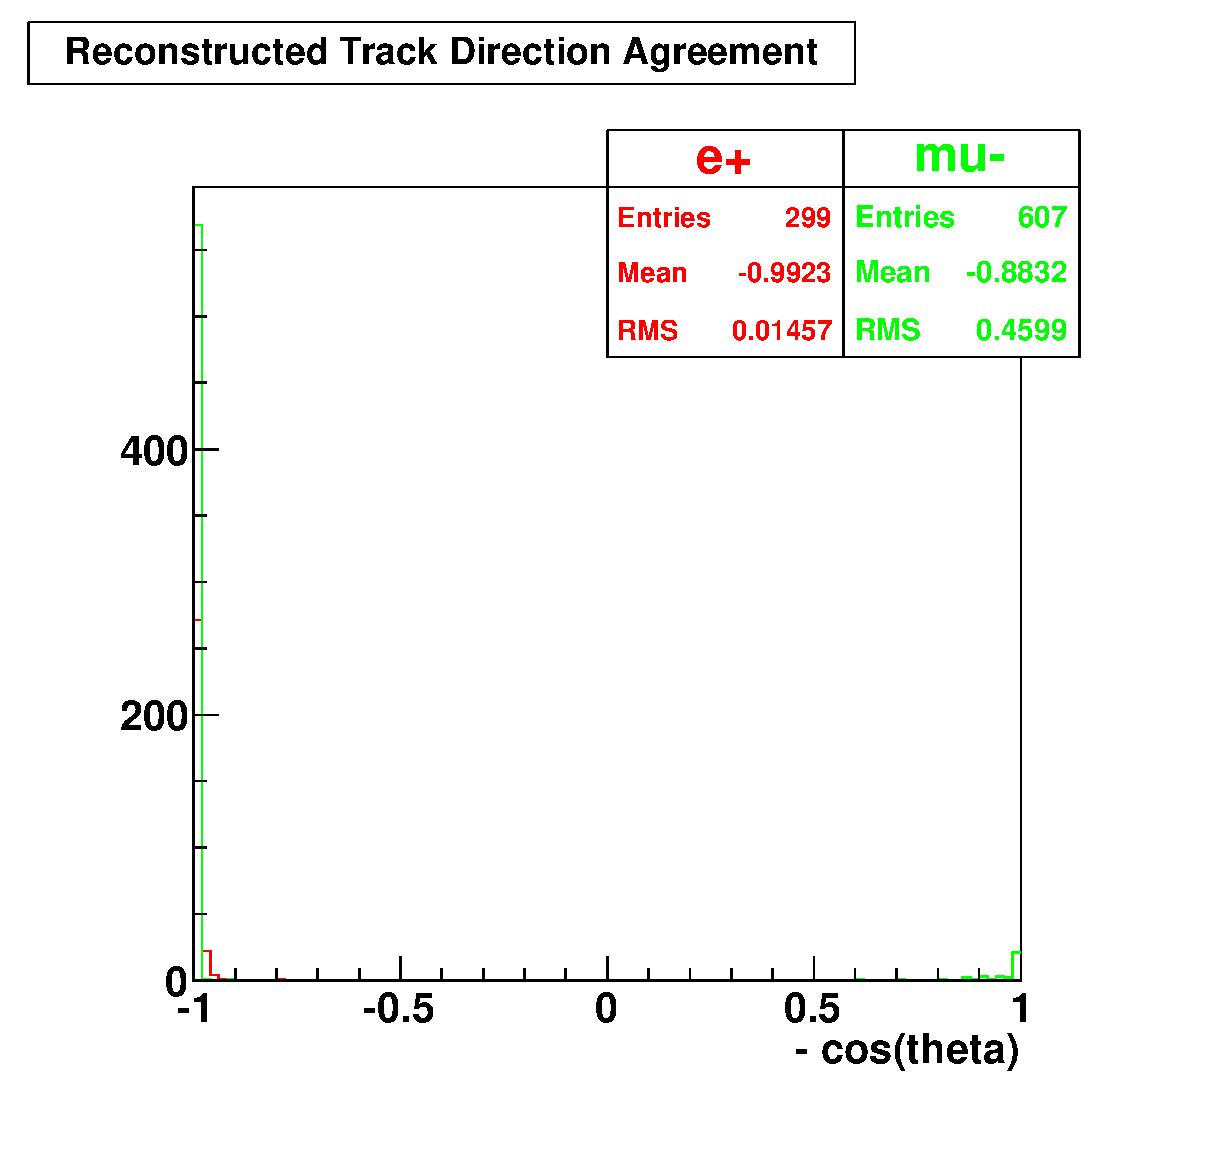
\includegraphics[width=\textwidth,height=0.9\textheight,keepaspectratio]
			{material/emu_mtq_recon_track_dir_agreement.pdf}
	\end{figure}
\end{frame}

\begin{frame}{Lepton Flavor Discrimination}
	\begin{figure}
		\includegraphics[width=\textwidth,height=0.9\textheight,keepaspectratio]
			{material/.pdf}
	\end{figure}
\end{frame}

\begin{frame}{Fully Contained T2K Event A}
	\begin{itemize}
		\item 76MeV
	\end{itemize}
	\begin{figure}
		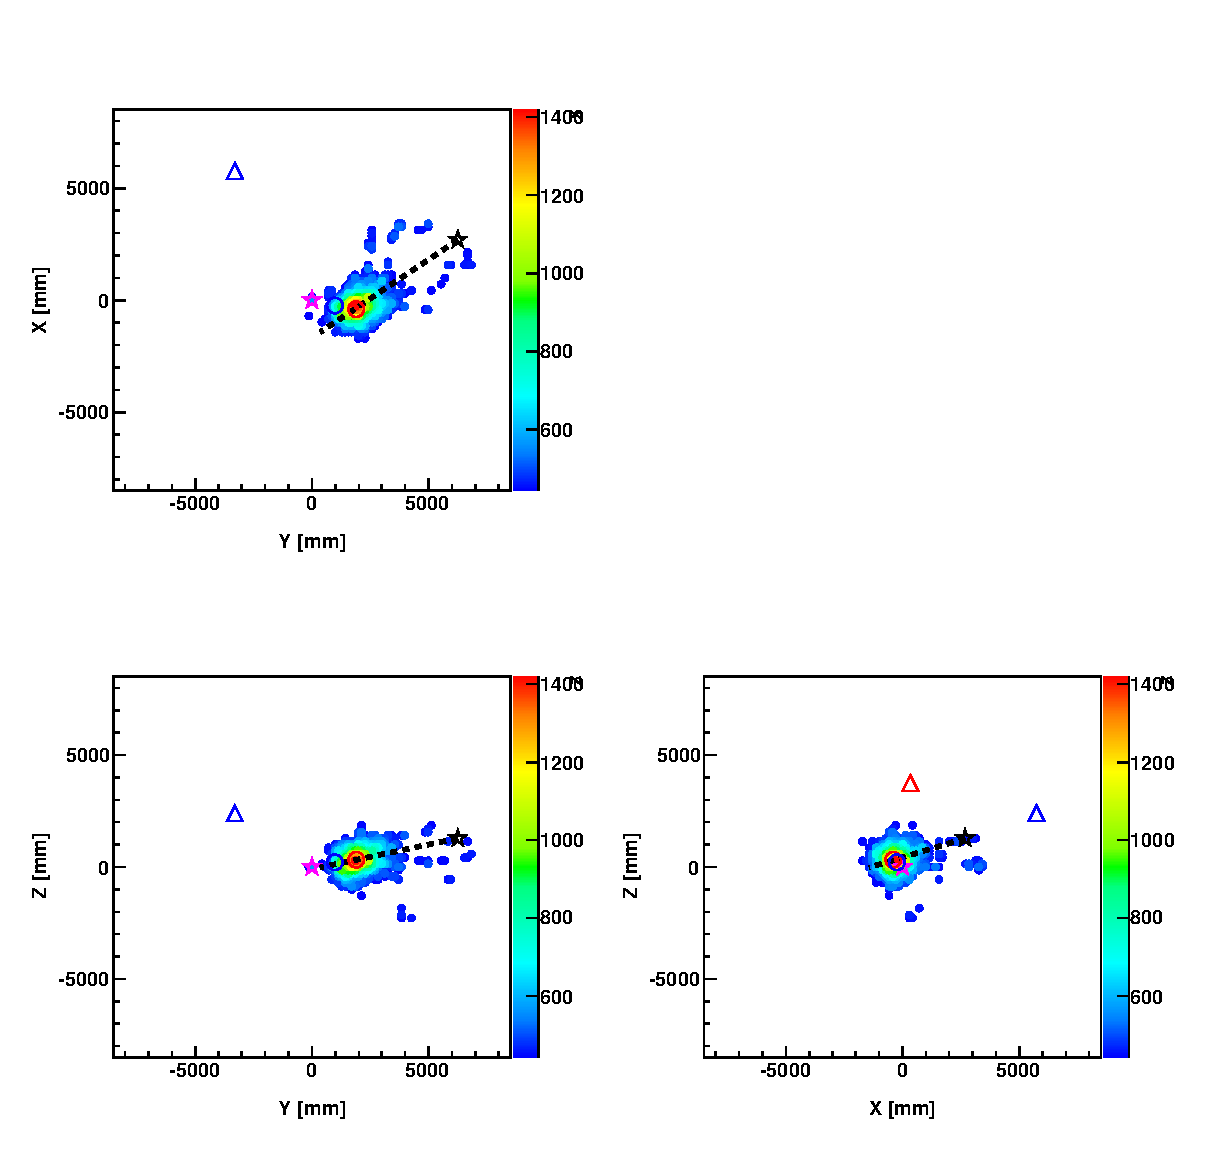
\includegraphics[width=\textwidth,height=0.9\textheight,keepaspectratio]
			{material/fom_map__run11331_evt29962767.pdf}
	\end{figure}
\end{frame}

\begin{frame}{Fully Contained T2K Event B}
	\begin{itemize}
		\item 131MeV
	\end{itemize}
	\begin{figure}
		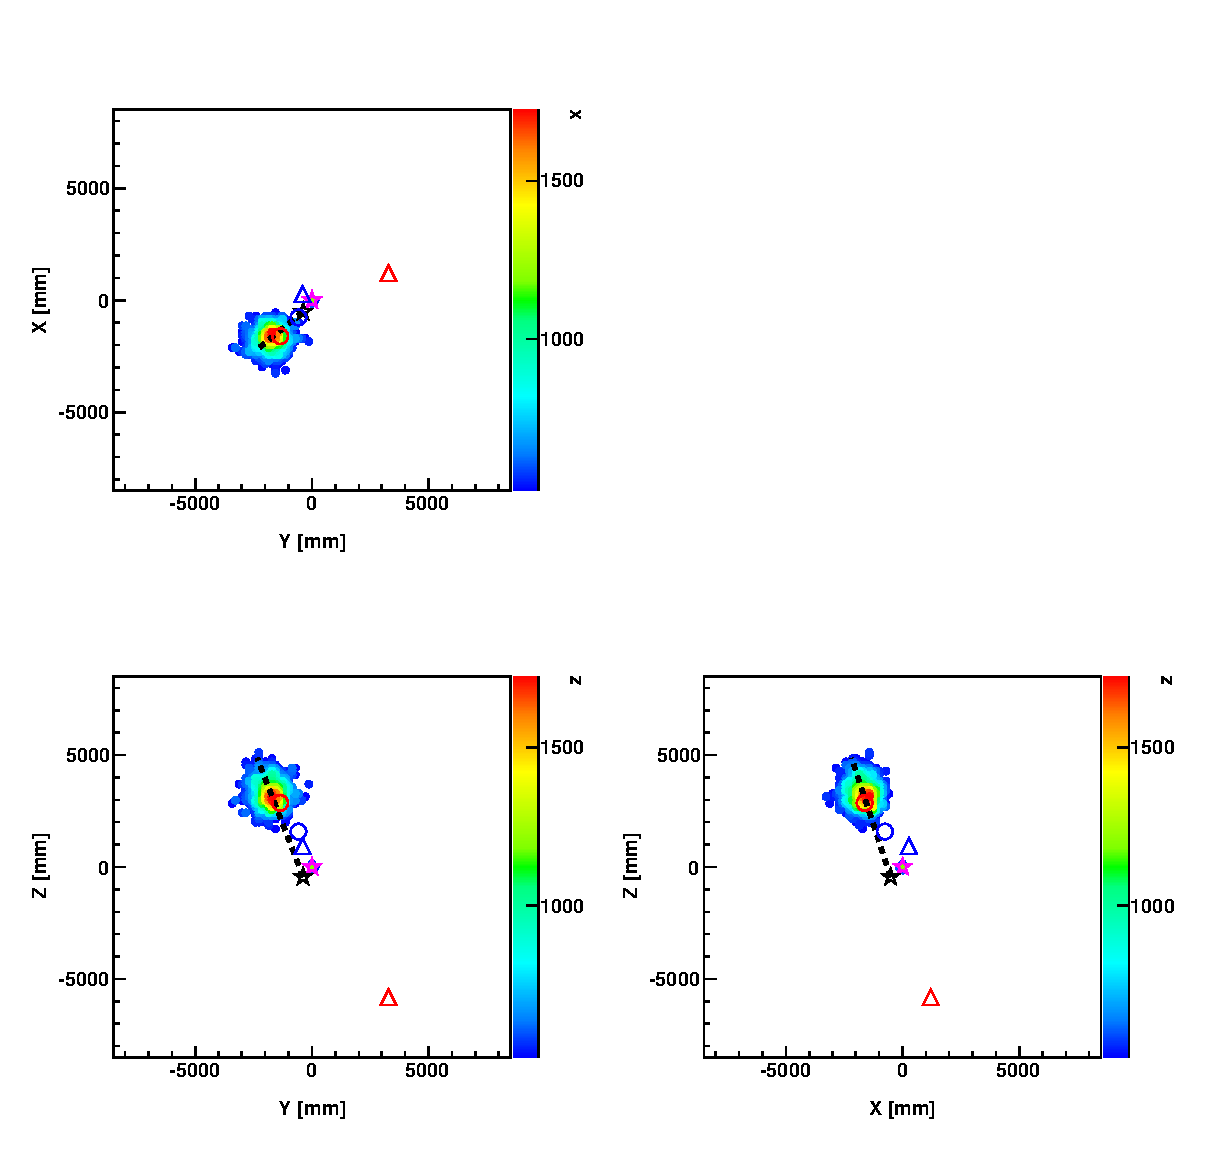
\includegraphics[width=\textwidth,height=0.9\textheight,keepaspectratio]
			{material/fom_map__run11317_evt8187014.pdf}
	\end{figure}
\end{frame}

\begin{frame}{Fully Contained T2K Event C}
	\begin{itemize}
		\item 363MeV
	\end{itemize}
	\begin{figure}
		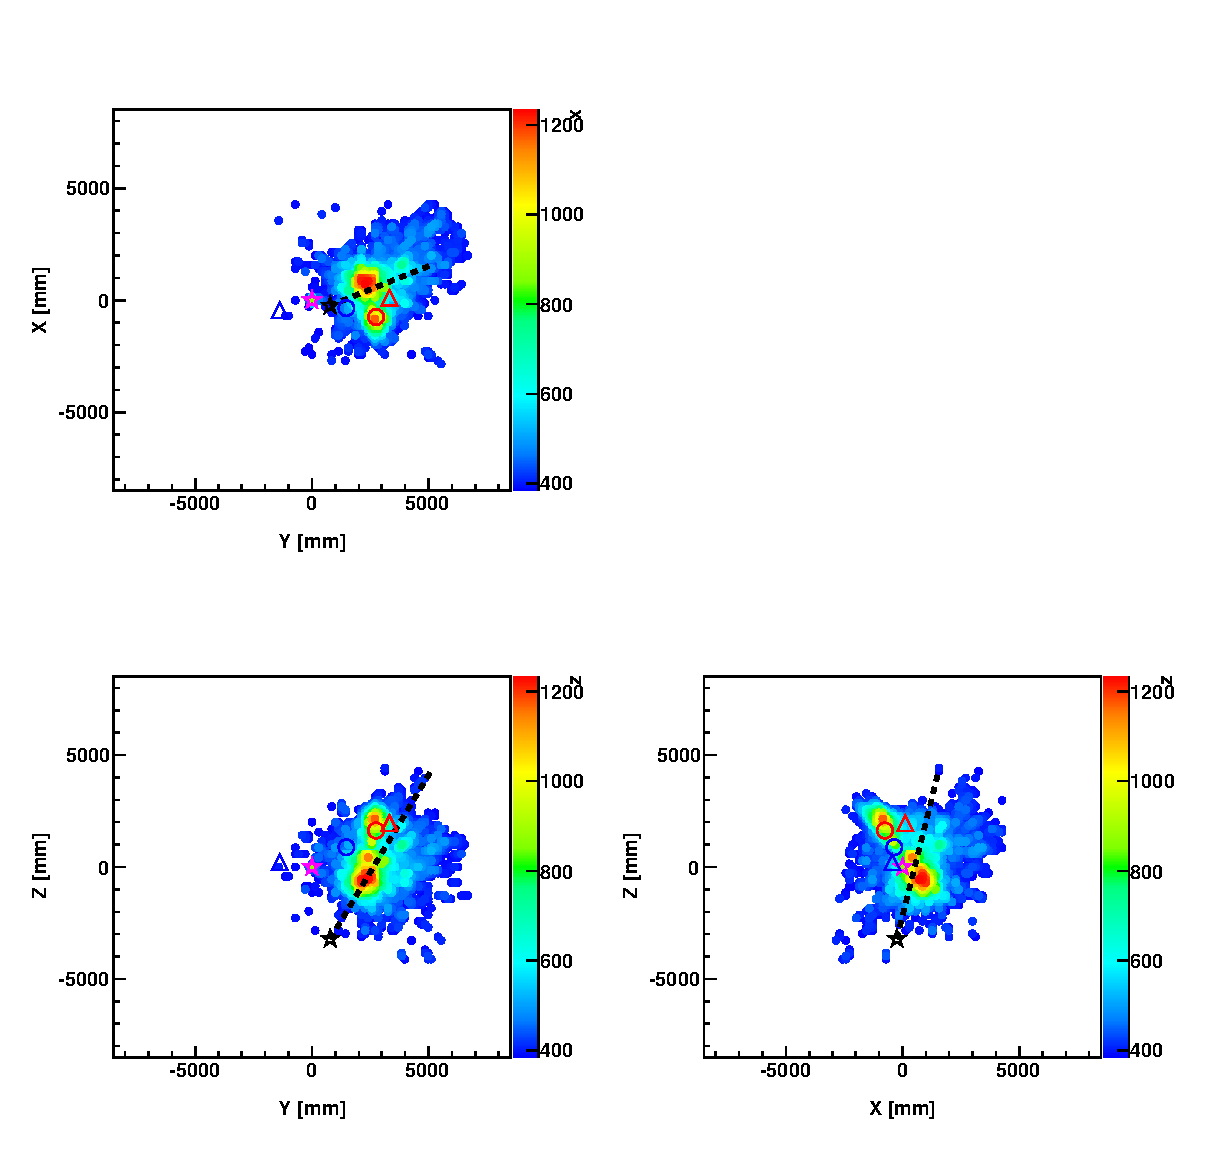
\includegraphics[width=\textwidth,height=0.9\textheight,keepaspectratio]
			{material/fom_map__run11339_evt39049330.pdf}
	\end{figure}
\end{frame}

\begin{frame}{T2K Event Direction}
	\begin{figure}
		\includegraphics[width=\textwidth,height=0.9\textheight,keepaspectratio]
			{material/.pdf}
	\end{figure}
\end{frame}

\begin{frame}{T2K Event $e/\mu$-like discrimination}
	\begin{figure}
		\includegraphics[width=\textwidth,height=0.9\textheight,keepaspectratio]
			{material/.pdf}
	\end{figure}
\end{frame}

\end{document}

\tikzstyle{na} = [baseline=-.5ex]

\begin{itemize}[<+-| alert@+>]
    \item Coriolis acceleration
        \tikz[na] \node[coordinate] (n1) {};
\end{itemize}

% Below we mix an ordinary equation with TikZ nodes. Note that we have to
% adjust the baseline of the nodes to get proper alignment with the rest of
% the equation.
\begin{equation*}
\vec{a}_p = \vec{a}_o+\frac{{}^bd^2}{dt^2}\vec{r} +
        \tikz[baseline]{
            \node[fill=blue!20,anchor=base] (t1)
            {$ 2\vec{\omega}_{ib}\times\frac{{}^bd}{dt}\vec{r}$};
        } +
        \tikz[baseline]{
            \node[fill=red!20, ellipse,anchor=base] (t2)
            {$\vec{\alpha}_{ib}\times\vec{r}$};
        } +
        \tikz[baseline]{
            \node[fill=green!20,anchor=base] (t3)
            {$\vec{\omega}_{ib}\times(\vec{\omega}_{ib}\times\vec{r})$};
        }
\end{equation*}

\begin{itemize}[<+-| alert@+>]
    \item Transversal acceleration
        \tikz[na]\node [coordinate] (n2) {};
    \item Centripetal acceleration
        \tikz[na]\node [coordinate] (n3) {};
\end{itemize}

% Now it's time to draw some edges between the global nodes. Note that we
% have to apply the 'overlay' style.
\begin{tikzpicture}[overlay]
        \path[->]<1-> (n1) edge [bend left] (t1);
        \path[->]<2-> (n2) edge [bend right] (t2);
        \path[->]<3-> (n3) edge [out=0, in=-90] (t3);
\end{tikzpicture}
